\section{Experiment 1}
	
	\textbf{Research Question:} When do Acoustic Classification tasks, learned in a deep learning multi-task, hard parameter sharing set-up, improve each other? 
	\textbf{Research Method:} Implement different multi-class acoustic classification tasks from different corpi and different domains as well as simpler auxiliary tasks specifically aimed at improving performance of the main task. The classification model will be a DNN without any adjustments for any specific task, to generalize the observations for task interaction in a multi-task learning setting. Different measurements are taken from the datasets beforehand. Each task is run in a single task set up, with different measurements being kept from the learning process and results. The goal of the investigation is to assess whether improved performance for one of the tasks in a dual task learning set-up can be predicted from the dataset and single inference task measurements through regression analysis.\\
	
	\textbf{Task choice:}\\
	
	Main Tasks\\
	
%	-- EXPLANATIONS OF TASKS\\
	\begin{itemize}
		\item General Acoustic Event Detection: Acoustic event detection or Sound event detection refers to the task of locating and classifying Sound Events in an audio from real life environments. General purpose AED means no specific optim
		\item Acoustic Scene Classification: Acoustic Scene Classification involves the automatic detection of the environment in an audio stream. Both indoor as well as outdoor environments can be included, with the length duration of a scene being long.
		\item Speaker Identification is the task of identifying the person speaking in an audio clip.
		\item Keyword Spotting aims at detecting predefined keywords in audio streams.
		\item Environmental Sound Classification (KEEP THIS FOR OTHER EXPERIMENT WHERE YOU INVESTIGATE DIFFERENT AED SETUPS like keeping out speech, polyphonic and monophonic, different datasets, specific vs non specific environment)
	\end{itemize}

%	-- REASONS WHY FOR THESE TASKS (use in other and general interest)\\
%	- Georgiev used them\\
%	- Most interesting for lifelogging purposes according to gurrin\\
%	- Different and multiple domains\\
%	- Domains: Speech, Environment, Music\\
%	- Different and multiple corpuses\\

	
	These are the main tasks, chosen to represent a variety of audio sensing tasks in the research. The tasks are more often then not the primary focus in audio sensing research, and are more complex in nature, with a multi-class classification goal. The choice was made for this specific set of tasks for multiple reasons. First of all, Gurrin et al. identified the main interests for audio sensing tasks for lifelogging purposes as being the identification of activities, audio events, location, people and keywords in dialogue, each of which is represented as a main task here. Futhermore, in work done by Georgiev, a system is built which combined Acoustic Scene Classification, Speaker Identification, Emotion Recognition and Stress detection, finding that all could be combined in a single multi-task DNN set-up without significant performance decrease. In this work the same DNN structure will as it has shown to perform well on multiple audio sensing tasks as well as allow direct verification for its findings. Furthermore are all (main and auxiliary) tasks chosen so that they would span multiple domains (Speech, Environment and Music), as well as multiple different datasets. 


	Auxiliary Tasks\\
	
	\begin{itemize}
		\item Music/Speech Detection
		\item Voice Activity Detection
		\item Emotion Detection
		\item Gender Detection
		\item Audio Tagging
		\item Event Activity Detection
		\item Stress Detection
		\item Music Instrument detection
	\end{itemize}
	
	
	%-- WHAT ARE AUXILIARY TASKS\\
	%- Smaller label set, simpler task\\
	%- Used to improve performance in other task\\
	%-- REASONS WHY FOR THESE TASKS (use in other and general interest)\\
	%- Used in literature\\
	%- M/S, Event activity detection and VAD used to explicitly learn how to differentiate between what is in the audio\\
	%- Emotion detection, stress detection and gender detection as semantic detection in speech domain, demonstrate whether it improves speech detection in other tasks, as well as performance of tasks in speech domain\\
%	- Music Instrument detection same as previous but for music domain\\
%	- Audio Tagging as a different specificity level compared to general audio event detection\\
%	-- REFER TO USE IN PAPERS\\
	
	The previous mentioned main tasks are supplemented by a list of auxiliary tasks, which are generally simpler tasks that are not often the main research goal but added as a side task to explicitly improve the main task. They often can be performed on the same dataset as the main task. Each task is treated as a main task and combined with all the other tasks. These are still mentioned as separate, as they are explicitly chosen for a specific relationship with at least one of the main tasks. Some tasks - e.g. Emotion detection - are also only considered auxiliary tasks in this context therefore. \\
	
	The reason for each inclusion will be disclosed next. There are three main categories the reasons of inclusion fall in, which relation to the main tasks this work aims to investigate: Simple differentiation, semantic detection in a specific domain and different specificity level. 
	
	\begin{itemize}
		\item With simple differentiation, the Music/Speech detection, Voice Activity Detection and Event Activity Detection tasks fall under this. These tasks simply try to differentiate if activity of a certain type is or isn't happening at a certain point. The hypothesis is that simple differentiation helps to build a representation that would make less errors for tasks where wrongfully differentiating the target labels of these tasks leads to prediction errors in its own results. 
		\begin{itemize}
			\item Music/Speech Detection: The task of classifying audio in a stream between Music, Speech or neither. This is included as it learns to differentiate between different domains which might be beneficial for all (main) tasks
			\item Voice Activity Detection: The task of detecting voice activity in a stream. This learns a representation that can differentiate specifically between what sound is or is not coming from a voice, which might lower the number of classification errors happening in SI and KS when the sound is not a voice, as well as AED for discriminating the speech label.
			\item Event Activity Detection: The task of detecting whether or not a sound event is happening at a certain point. In the literature (REFERENCE) AED has often been defined as a multi-task problem, by splitting the tasks of detecting an event and determining the type of event (Audio Tagging) in two, while still learning them simultaneously and combining the results afterwards. This has lead to better performance to baseline single task AED systems. This inclusion might be beneficial for lowering detection errors when no (target) sound event is present AED, SI and KS. 
		\end{itemize}
	
		\item Next is semantic detection, which here means the Emotion detection, stress detection, gender detection in the speech domain and music instrument detection in the music domain. These try to identify a certain property of events in the audio. The idea of including this is to check whether identifying more complex properties of speech and music having a less direct link to the purposes of the main tasks can be beneficial for performance.
		\begin{itemize}
			\item Emotion Detection: The task of detecting emotion from speech and music. This was included in the work done by Georgiev as well as others. Emotion Detection is not expected to have any direct link to any of the main tasks, except perhaps a loose one with the speech domain tasks. 
			\item Gender Detection: The task of detecting gender of a speaker. This is directly linked to speaker identification, as the same speaker will have the same gender. 
			\item  Stress Detection: The task of detecting stress in speech audio. This was also included in the work done by Georgiev. Stress detection has a loose connection with the speech domain, but a direct one with Emotion Detection. It has a smaller target labelset size than Emotion Detection, in which we are interested due to previous observations that tasks with smaller target label sets make for better auxiliary tasks.
			\item  Music Instrument detection: The task of detecting which music instrument is played in an audio clip. This has a loose connection with the music domain, which might be interesting for better detection of music audio, leading to less wrongful labels for events that are out of target for the main tasks.
		\end{itemize}
	
		\item The last one is different specificity level, under which only audio tagging falls directly, as it is a simpler version of AED (you only need to identify what is happening in the whole clip and not when it is or is not present). The first category can be seen as a more specific subset of this with a small target label set though. The interest for this class is different, in the sense that it is more about reporting the difference adding a simplified version of the same task makes as well as comparing its interaction with the other tasks to the specific version.
		\begin{itemize}
			\item Audio Tagging: In AED research, improved results have been achieved by defining the task of AED as two separate tasks, namely Audio Tagging and Event Activity Detection, learned simultaneously in a multi-task framework. Besides this, work done by Huang et al. achieved the best results in the 2019 AED challenge by adding additional branches of audio tagging tasks (with different pooling methods) besides the main Audio Tagging/Event Detection branch. Therefore the interest lies in its comparison with the performance compared to single task AED as well as its interaction with other tasks in a multi-task framework.
		\end{itemize}
	\end{itemize}
	
	\begin{table}[ht]
		\caption{Tried Combinations} % title of Table
		\centering % used for centering table
		\begin{tabular}{p{0.2\textwidth}p{0.6\textwidth}p{0.2\textwidth}} % centered columns (4 columns)
			\hline\hline %inserts double horizontal lines
			Title & Tasks & Classifier   \\ [0.5ex] % inserts table
			%heading
			\hline % inserts single horizontal line
			\citet{lu2004multitask} & Automatic Speech Recognition; Speech Enhancement; Gender Detection & RNN \\ \hline
			\citet{panchapagesan2016multi} & Keyword Spotting; Large Vocabulary Continuous Speech Recognition Senones Targets Recognition & \\ \hline
			\citet{sakti2016deep} & Automatic Speech Recognition; Acoustic Event Detection & DNN \\ \hline
			\citet{georgiev2017heterogeneous} \citet{georgiev2017low} & Speaker Identification; Emotion Detection; Stress Detection; Acoustic Scene Classification & DNN \\ \hline
			\citet{kim2017speech} & Emotion Detection; Auxiliary tasks: Arousal Level; Valence Level; Gender Detection & CNN \\ \hline
			\citet{nwe2017convolutional} & Acoustic Scene Classification (Grouped scenes as different tasks) & \\ \hline
			\citet{sun2017compressed} & Keyword Spotting; Large Vocabulary Continuous Speech Recognition Phone Targets Recognition & \\ \hline
			\citet{kremer2018inductive} & Word Error Rate and Character-Level Automatic Speech Recognition & CNN \\ \hline
			\citet{morfi2018deep} & Audio Tagging; Event Activity Detection & DNN \\ \hline
			\citet{lee2019label} & Main Tasks: Audio Tagging; Speaker Identification; Speech Command Recognition (Keyword Spotting); Auxiliary Tasks: Next-Step prediction; Noise Reduction; Upsampling &  \\ \hline
			\citet{lopez2019keyword} & Keyword Spotting; Own-voice/External Speaker Detection & \\ \hline
			\citet{pankajakshan2019polyphonic} & Sound Activity Detection (Event Activity Detection); Sound Event Detection (Audio Tagging) & CRNN \\ \hline
			\citet{tonami2019joint} & Acoustic Event Detection; Acoustic Scene Classification & CRNN for AED, CNN for ASC  \\ \hline
		\end{tabular}
		\label{table:combinations} % is used to refer this table in the text
	\end{table}

	\begin{table}[ht]
		\caption{Tried Combinations (Continued)} % title of Table
		\centering % used for centering table
		\begin{tabular}{p{0.2\textwidth}p{0.6\textwidth}p{0.2\textwidth}} % centered columns (4 columns)
			\hline\hline %inserts double horizontal lines
			Title & Tasks & Classifier   \\ [0.5ex] % inserts table
			%heading
			\hline % inserts single horizontal line
			\citet{xia2019multi} & Acoustic Event Type Detection (Audio Tagging); Predict frame position information (Event Activity Detection) & CNN \\ \hline
			\citet{xu2019multi} & Acoustic Event Detection; Acoustic Scene Classification & \\ \hline
			\citet{zeng2019spectrogram} (1) & Emotion Detection; Music/Speech Classification & DNN \\ \hline
			\citet{zeng2019spectrogram} (2) & Accent Recognition; Speaker Identification & DNN \\ \hline
			\citet{abrol2020learning} & Fine and Coarse Labels Acoustic Scene Classification & DNN \\ \hline
			\citet{deshmukh2020multi} & Acoustic Event Detection; Reconstruct Time Frequency Representation of Audio &  CNN \\ \hline
			\citet{fernando2020temporarily} & Acoustic Event Type Detection (Audio Tagging); Predict Frame Position Information (Event Activity Detection) & LSTM \\ \hline
			\citet{huang2020guided} & Audio Tagging; Temporal Detection (Event Activity Detection) & CNN PT/PS model \\ \hline
			\citet{huang2020multi} & Audio Tagging; Event Boundary Detection (Event Activity Detection) & CNN \\ \hline
			\citet{tagliasacchi2020multi} & Keyword Spotting; Speaker Identification; Language Identification; Music/Speech Classification; Bird Audio Detection; Urban Acoustic Scene Classification; Music Instrument Pitch Detection; Music Instrument Detection & CNN  \\ \hline
			\citet{wu2020domain} & Keyword Spotting; Domain Prediction & \\
			[1ex] % [1ex] adds vertical space
			\hline %inserts single line
		\end{tabular}
		\label{table:combinations2} % is used to refer this table in the text
	\end{table}


	% This might be a different research question:
	% - How does splitting up AED in EAD and AT tasks affect the multi-task set-up?
	% - How does a general AED into different set-ups affect the multi-task set-up?

	% \textbf{Literature Observations:}\\
	
	
	\textbf{Neural Network:}\\
	%-- REFER TO GEORGIEV'S USE AND NLP RESEARCH JUSTIFICATION FOR USING 1\\
	
	\begin{figure}
		\centering
		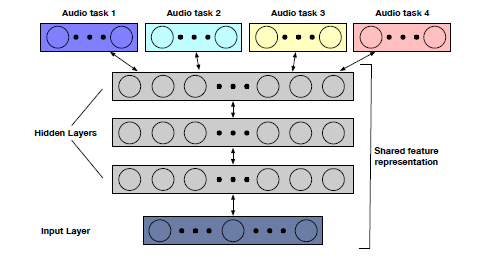
\includegraphics[width=0.9\linewidth]{NN.PNG}
		\caption{Multi-task DNN model}
		\label{fig:NN}
	\end{figure}

	%Basis: DNN feed-forward propagation classifier
	%Input: Statistical summaries of log filter banks
	%Architecture: Input and hidden layers are shared across potential combinations of audio analysis tasks -> Universal feature transformation that captures acoustic observations. 3 hidden layers with either 128, 256 or 512 nodes each, hard parameter sharing. Soft-max layer at the task-specific layers, updated separately depending on the training input instance.
	%Training: mini-batch stochastic gradient descent all audio tasks simultaneously
	%Fine-tuning: backpropagation
	%Additional: Keep the hyper-parameters fixed across single-task and multi-task settings for comparison. Use fixed random seed set upfront to facilitate replicability. Do not use any task-specific features or pre-trained embeddings for initialisation to delimit the behaviour of the architecture and analyse the interaction between tasks.
	
	The architecture is based on the system, described by \citet{georgiev2017heterogeneous}, which is a Deep Neural Network (DNN) feed-forward propagation classifier. As seen in figure \ref{fig:NN}, in a multi-task setting, all tasks share the same input and hidden layers, with task-specific output layers. This leads to these layers being used as a universal feature transformation which captures acoustic observations from different tasks. For the input, features have to be extracted from the audio. In the original work this is implemented by statistical summaries of log filter banks, extracted from each audio frame. They use summaries both for reducing the input feature complexity as well as allowing a representation of the same size across multiple tasks. \\
	
	To allow for comparison and analysis of the interaction between tasks, this work follows the approach from \cite{alonso2016multitask} and \cite{bingel2017identifying} the hyperparameters (this includes a fixed random seed set) and the architecture will be kept the same, regardless of which and the number of tasks learned. The set-up \citet{georgiev2017heterogeneous} had was 3 hidden layers which were tested at 128, 256 or 512 in each layer, with a soft-max pooling layer at the output layers. The output layers are updated separately depending on whether the training input instance is one for their own task. Furthermore, no task-specific features, nor any pre-trained embeddings will be used for initialisation to avoid any task bias. \\
	
	The training is done by mini-batch Stochastic Gradient Descent (SGD) on all audio tasks simultaneously, which is the key to succesfully training the multi-task DNN \citep{georgiev2017heterogeneous}. The samples are randomised across tasks before being fed into the DNN system. Backpropagation is then used for the fine-tuning of the DNN, which again only trains the softmax layer for the task at hand with the other softmax layers being kept intact. \\
	
	This set-up is chosen for the same reasons as Georgiev, namely due to the fact that it proved to be successful in multiple audio analysis tasks, as well as providing a good comparison opportunity for analysing the results. As \citet{bingel2017identifying} noted in their work as well however, the fixed hyper-parameters make the results only applicable to the scenario where one wants to know whether MTL works in the chosen parameter configuration.\\
	
	\textbf{Dataset measurements:}\\
	One way of structurally figuring out when multiple tasks can improve each other is described in \citet{alonso2016multitask} and \citet{bingel2017identifying}, where they try to predict which dataset and task features correlate to improvements in the multi-task setting for NLP tasks. \citet{bingel2017identifying} builds a regression analysis system for this to find the Pearson Coefficiënt between pre-measured data and the change in F1 score from single to multi-task systems. There are 3 groups of dataset measurements which will be examined: Dataset features, Information Theory derived features and Single task inference features. \\
	
	\textbf{Dataset features}
	\begin{itemize}
		\item Number of labels
		\item Number of clips
		\item Number of labeled frames
		\item Type/token ratio
		\item Labels per domain
		\item Dataset size
	\end{itemize}
	
	\textbf{Information Theory derived features}
	
	In \citet{alonso2016multitask}, these were found to be the most informative features. The interest is in determining whether these results are transferable to the audio domain.
	\begin{itemize}
		\item label entropy: Entropy of the label distribution
		\item label kurtosis: Indicates the skewness of a distribution
	\end{itemize}
	
	\textbf{Learning curve features}
	
	In \citet{bingel2017identifying} these were one of the most informative features. This involves taking measurements of the learning curve for the single tasks at different stages.
	\begin{itemize}
		\item Curve gradients: The gradients of the loss curve, taken at 10, 20, 30, 50 and 70 percent of the total number of batches
		\item Fitted log-curve: A logarithmic functio is fitted to the loss curve values, where the function is of the form L(i) = a*ln(c*i+d) + b where a and c are features that describe the steepness of the learning curve.
	\end{itemize}		
	
	\textbf{Audio features}
	
	Along with the features from the NLP research, additional audio related features are taken in account, which have been mentioned in the literature.
	\begin{itemize}
		\item Average sample length
		\item Total length of dataset (in seconds)
		\item Sampling rate
		\item Signal to Noise Ratio
	\end{itemize}
	
	\textbf{Non-numetric Factors}
	
	Finally there are also non-numetric Factors that might have an impact. 
	\begin{itemize}
		\item Overlapping\\Non-overlapping events
		\item Unlabeled, weakly labeled and strongly labeled dataset
		\item Mono or Stereo channel
	\end{itemize}
	
	\textbf{Evaluation:}\\
	
	The evaluation will 
	
	For evaluation these are the general metrics
	
	\begin{itemize}
		\item Averaged F1 score: The event categories are considered equally important \cite{phan2019unifying}
		\item Overall F1 score: The event instances are considered equally important \cite{phan2019unifying}
		\item Accuracy: Used in contexts where false positives and false negatives are less important than the rate of true positives and true negatives, which is often the case in audio sensing tasks.
		\item Detection Error Rate (ER): Used for evaluating correct segmentation of events from a continuous test signal \cite{phan2019unifying}
		\item Area Under the Receiver Operating Characteristic Curve (ROC AUC): plots the true positive rate against the false positive rate, with the metric being calculated from the area under the plot. Random guesses have an AUC of 0.5 \cite{deshmukh2020multi}
		\item Pearson coefficient: Measure for correlation between two variables. In this case, this will be the correlation of the numeric measurements from the dataset. For this a regression analysis system will be built.
		\item Intermediate output variances: Used in \cite{xia2019multi}  (to prove they can average respective noise patters, see 2020 Xia et al.)
		%\item Ablation Model of input embeddings to evaluate discriminative feature learning (see 2020 Fernando, 2020 Deshmukh et al.) different experiment
		%\item SNR (see 2016 Sakti et al.) Different experiment
		\item Efficiency: Combining tasks in a multi-task setting is used both for performance as efficiency purposes. Two metrics will be evaluated, following \cite{georgiev2017heterogeneous}. Both of these will be compared to running a single inference task and the combined time of running all combined tasks separately.
		\begin{itemize}
			\item Runtime: The time needed for performing audio classification 
			\item Memory: The size of the trained multi-task DNN compared to the single task and combined single tasks variants.
		\end{itemize}
	\end{itemize}

	Lastly, this work will take a look at class relationships in the context of multi-task. In the research, a few observations have already been made, in regards to the effect of the combination of tasks on certain classes. Specifically in this experiment, two effects will be specifically investigated. 
	
	\begin{itemize}
		\item \textbf{Speech related tasks for AED}: (REFERENCE) multiple observations have been made that for a general AED classifier, the Speech class is often mislabeled and causes mislabels of events like coughs. (CITE) notes that this is due to the fact that speech signals and environmental audio signals have a different structure. Therefore, this experiment especially interested in whether and/or which tasks in the speech domain can improve the speech class detection in AED. 
		\item \textbf{AED events only happening in certain scenes for ASC}: (REFERENCE) has noticed, when combining AED and ASC that AED can improve ASC, especially when certain events only happen in specific scenes. This was also found to go in the other direction, namely that events happening in multiple scenes will lead to a worse performance in ASC. This means the overview will be made of which events are in which scenes and also which ones are unique. 
	\end{itemize}
